% Simplified diagram of the quotient digit table (pla.vhd).
%
% The horizontal axis is the divisor d, and the vertical axis is the partial
% remainder n. The staircases are the boundaries between the quotient digits
% selected by the table. They are generated by "./srt.py --tikz", see the
% Makefile.
%
% Build with "make pla.svg".

\documentclass[tikz,border=6pt]{standalone}

\begin{document}
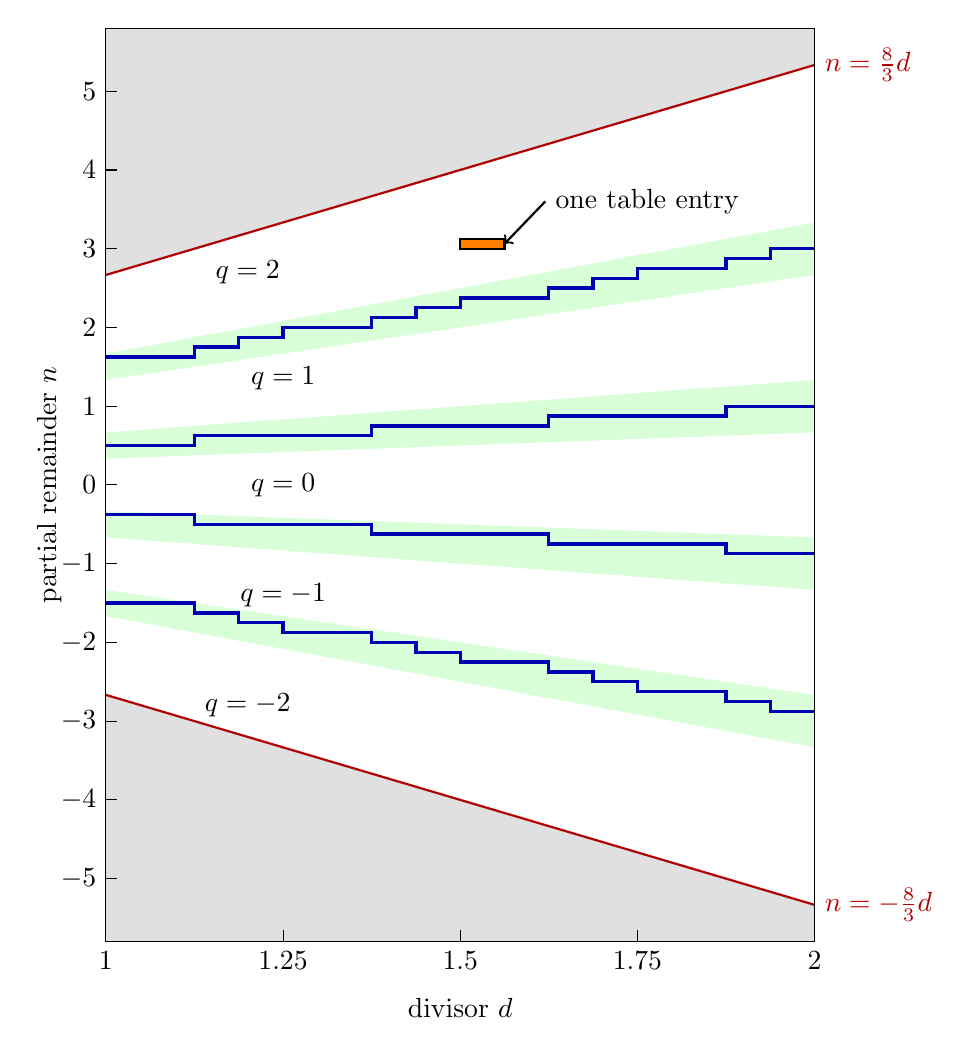
\begin{tikzpicture}[x=9cm, y=1cm,
                    boundary/.style={very thick, blue!70!black},
                    bound/.style={thick, red!70!black},
                    band/.style={fill=green!15},
                    outside/.style={fill=black!12}]

   % The region outside the bound |n| <= 8d/3, which is never reached
   \fill[outside] (1, 8/3) -- (2, 16/3) -- (2, 5.8) -- (1, 5.8) -- cycle;
   \fill[outside] (1, -8/3) -- (2, -16/3) -- (2, -5.8) -- (1, -5.8) -- cycle;

   % The bands where both digit k and k+1 are allowed: (k+1/3)d <= n <= (k+2/3)d
   \foreach \k in {-2, -1, 0, 1} {
      \fill[band] (1, \k + 1/3) -- (2, 2*\k + 2/3) -- (2, 2*\k + 4/3) -- (1, \k + 2/3) -- cycle;
   }

   % The bound |n| <= 8d/3
   \draw[bound] (1, 8/3) -- (2, 16/3) node[right] {$n = \frac{8}{3}d$};
   \draw[bound] (1, -8/3) -- (2, -16/3) node[right] {$n = -\frac{8}{3}d$};

   % The boundaries between the digits selected by the table
   % Generated by ./srt.py --tikz. Do not edit.
\draw[boundary] (1,-1.5) -- (1.0625,-1.5) -- (1.0625,-1.5) -- (1.125,-1.5) -- (1.125,-1.625) -- (1.1875,-1.625) -- (1.1875,-1.75) -- (1.25,-1.75) -- (1.25,-1.875) -- (1.3125,-1.875) -- (1.3125,-1.875) -- (1.375,-1.875) -- (1.375,-2) -- (1.4375,-2) -- (1.4375,-2.125) -- (1.5,-2.125) -- (1.5,-2.25) -- (1.5625,-2.25) -- (1.5625,-2.25) -- (1.625,-2.25) -- (1.625,-2.375) -- (1.6875,-2.375) -- (1.6875,-2.5) -- (1.75,-2.5) -- (1.75,-2.625) -- (1.8125,-2.625) -- (1.8125,-2.625) -- (1.875,-2.625) -- (1.875,-2.75) -- (1.9375,-2.75) -- (1.9375,-2.875) -- (2,-2.875);
\draw[boundary] (1,-0.375) -- (1.0625,-0.375) -- (1.0625,-0.375) -- (1.125,-0.375) -- (1.125,-0.5) -- (1.1875,-0.5) -- (1.1875,-0.5) -- (1.25,-0.5) -- (1.25,-0.5) -- (1.3125,-0.5) -- (1.3125,-0.5) -- (1.375,-0.5) -- (1.375,-0.625) -- (1.4375,-0.625) -- (1.4375,-0.625) -- (1.5,-0.625) -- (1.5,-0.625) -- (1.5625,-0.625) -- (1.5625,-0.625) -- (1.625,-0.625) -- (1.625,-0.75) -- (1.6875,-0.75) -- (1.6875,-0.75) -- (1.75,-0.75) -- (1.75,-0.75) -- (1.8125,-0.75) -- (1.8125,-0.75) -- (1.875,-0.75) -- (1.875,-0.875) -- (1.9375,-0.875) -- (1.9375,-0.875) -- (2,-0.875);
\draw[boundary] (1,0.5) -- (1.0625,0.5) -- (1.0625,0.5) -- (1.125,0.5) -- (1.125,0.625) -- (1.1875,0.625) -- (1.1875,0.625) -- (1.25,0.625) -- (1.25,0.625) -- (1.3125,0.625) -- (1.3125,0.625) -- (1.375,0.625) -- (1.375,0.75) -- (1.4375,0.75) -- (1.4375,0.75) -- (1.5,0.75) -- (1.5,0.75) -- (1.5625,0.75) -- (1.5625,0.75) -- (1.625,0.75) -- (1.625,0.875) -- (1.6875,0.875) -- (1.6875,0.875) -- (1.75,0.875) -- (1.75,0.875) -- (1.8125,0.875) -- (1.8125,0.875) -- (1.875,0.875) -- (1.875,1) -- (1.9375,1) -- (1.9375,1) -- (2,1);
\draw[boundary] (1,1.625) -- (1.0625,1.625) -- (1.0625,1.625) -- (1.125,1.625) -- (1.125,1.75) -- (1.1875,1.75) -- (1.1875,1.875) -- (1.25,1.875) -- (1.25,2) -- (1.3125,2) -- (1.3125,2) -- (1.375,2) -- (1.375,2.125) -- (1.4375,2.125) -- (1.4375,2.25) -- (1.5,2.25) -- (1.5,2.375) -- (1.5625,2.375) -- (1.5625,2.375) -- (1.625,2.375) -- (1.625,2.5) -- (1.6875,2.5) -- (1.6875,2.625) -- (1.75,2.625) -- (1.75,2.75) -- (1.8125,2.75) -- (1.8125,2.75) -- (1.875,2.75) -- (1.875,2.875) -- (1.9375,2.875) -- (1.9375,3) -- (2,3);


   % One table entry, i.e. n in [3, 3+1/8) and d in [1.5, 1.5+1/16)
   \draw[thick, fill=orange] (1.5, 3) rectangle (1.5625, 3.125);
   \draw[<-, thick] (1.5625, 3.0625) -- (1.62, 3.6) node[right] {one table entry};

   % The quotient digits
   \node at (1.2, 2.7)   {$q = 2$};
   \node at (1.25, 1.35) {$q = 1$};
   \node at (1.25, 0)    {$q = 0$};
   \node at (1.25, -1.4) {$q = -1$};
   \node at (1.2, -2.8)  {$q = -2$};

   % Axes
   \draw (1, -5.8) rectangle (2, 5.8);
   \foreach \d in {1, 1.25, 1.5, 1.75, 2} {
      \draw (\d, -5.8) -- (\d, -5.65);
      \node[below] at (\d, -5.8) {\d};
   }
   \foreach \n in {-5, ..., 5} {
      \draw (1, \n) -- (1.015, \n);
      \node[left] at (1, \n) {$\n$};
   }
   \node[below] at (1.5, -6.4) {divisor $d$};
   \node[rotate=90] at (0.92, 0) {partial remainder $n$};

\end{tikzpicture}
\end{document}
